%\section{Instrumentos}

	\par Os instrumentos de pesquisa existem para que se possam levantar
informações para realizar um determinado projeto.

	\par Pode-se dizer que um questionário é uma forma de coletar
informações através de algumas perguntas feitas a um público específico.
Segundo \citeonline{gunther2003}, o questionário pode ser definido como
um conjunto de perguntas que mede a opinião e interesse do respondente.

	\par Neste trabalho foi realizado um questionário simples, apresentado na
Figura \ref{fig:qm1}, contendo quatro perguntas e enviado para \textit{e-mails}
de alguns alunos da universidade. O foco desse questionário foi saber o motivo
pelo qual os usuários mais acessavam o portal do aluno e se tinham alguma
dificuldade em encontrar o que procuravam. Obteve-se um total de treze
respostas, no qual pode-se perceber que a maioria dos entrevistados afirmou
ter dificuldades para encontrar as informações de que necessitam, e que
gostariam de ser notificados quando houvesse alguma atualização de notas. Sobre
o motivo do acesso, cem por cento dos discentes responderam que entram no
sistema \textit{web} para consultar os resultados das avaliações.

	\begin{figure}[h!]
		\centerline{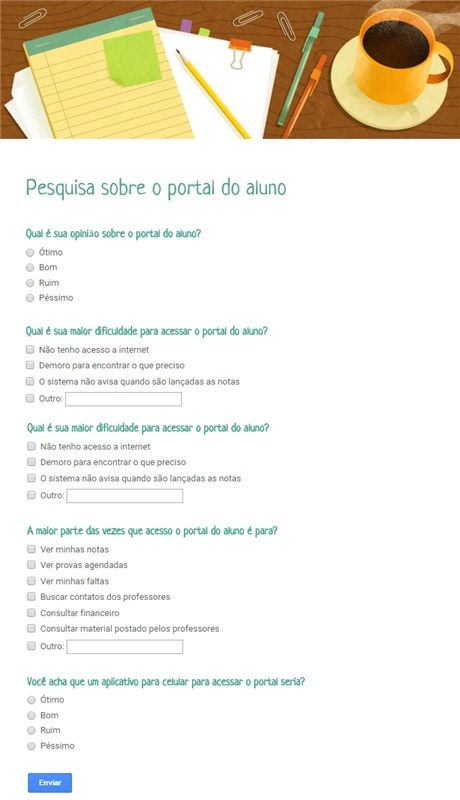
\includegraphics[scale=1]{./imagens/2_q_metodologico/3_instrumentos/instrumentos.png}}
		\caption[Quetionário Aplicado]{Quetionário Aplicado.
			\textbf{Fonte:}Elaborado pelos autores.}
		\label{fig:qm1}
	\end{figure}
	
	
	

	\par Outro instrumento utilizado para realizar esta pesquisa foram as reuniões,
ou seja, reunir-se com uma ou mais pessoas em um local, físico ou remotamente
para tratar algum assunto específico. Para \citeonline{ferreira1999}, reunião é o ato de
encontro entre algumas pessoas em um determinado local, com finalidade de tratar
qualquer assunto.

	\par Durante a pesquisa, foram realizadas reuniões entre os participantes com
o objetivo de discutir o andamento das tarefas as quais cada integrante
responsabilizou-se a fazer, além de traçar novas metas. Também foram utilizadas
referências de livros, revistas, manuais e \textit{web sites}.

\pagebreak